\documentclass[11pt]{article}
\usepackage[margin=1in]{geometry}
\usepackage{amsmath,amssymb,amsthm,mathtools}
\usepackage{graphicx}
\usepackage{microtype}
\usepackage[colorlinks=true,linkcolor=blue,citecolor=blue,urlcolor=blue]{hyperref}
\newtheorem{theorem}{Theorem}
\newtheorem{lemma}[theorem]{Lemma}
\newtheorem{remark}[theorem]{Remark}
\newcommand{\whot}{\widehat{\otimes}}
\newcommand{\ellone}{\ell^{1}}
\newcommand{\B}{\mathcal B}
\newcommand{\A}{\mathcal A}
\newcommand{\id}{\mathrm{id}}
\title{Amenability of a twisted \(\ell^1\)-crossed product\\forces amenability of the acting group}
\author{Solution packet for arXiv:1705.02623}
\date{27 August 2026}

\begin{document}
\maketitle

\begin{abstract}
De Jeu, El Harti and Pinto ask whether amenability of
\(\ellone(G,A;\alpha)\), for a discrete group \(G\) and a nonzero
\(C^*\)-algebra \(A\), forces \(G\) to be amenable.  We prove that it does.
In fact, the \(C^*\)-structure is unnecessary: the conclusion holds for
every nonzero Banach algebra acted on isometrically by \(G\).  The proof
turns a multiplier-central approximate diagonal into a Reiter \(P_1\) net
by retaining its \((p,p^{-1})\)-coefficients.
\end{abstract}

\section{The source problem and the answer}

For an action \(\alpha:G\to\operatorname{Aut}(A)\) of a discrete group by
isometric automorphisms, write
\[
 \B=\ellone(G,A;\alpha),\qquad
 (f*h)(r)=\sum_{s\in G}f(s)\alpha_s\bigl(h(s^{-1}r)\bigr).
\]
Section 5 of \cite{source} asks whether amenability of \(\B\), for nontrivial
\(A\), implies amenability of \(G\).  The exact statement appears on source
PDF page 16:

\begin{center}
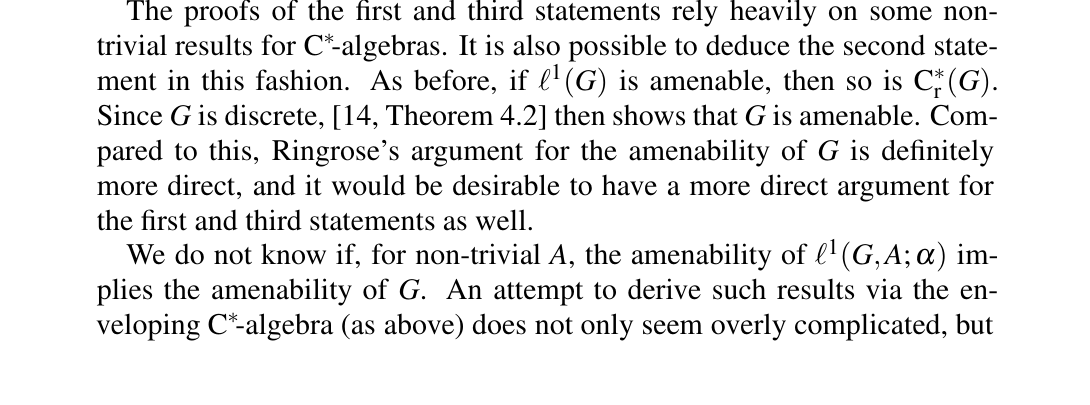
\includegraphics[width=0.96\textwidth]{figures/open_question_crop.png}
\end{center}

\begin{theorem}[Full answer, in stronger form]\label{thm:main}
Let \(A\ne\{0\}\) be a Banach algebra and let the discrete group \(G\) act
on \(A\) by isometric algebra automorphisms.  If
\(\ellone(G,A;\alpha)\) is an amenable Banach algebra, then \(G\) is an
amenable group.
\end{theorem}

This applies in particular to every nontrivial \(C^*\)-dynamical system in
the question.  No unit, character, invariant state, positivity, separability,
or countability assumption is needed.

\section{Proof intuition}

An approximate diagonal for \(\B\) is a family of two-variable coefficient
tensors.  The group itself acts on \(\B\) by canonical left and right
multipliers, even if \(A\) has no unit.  Amenability lets us choose the
diagonal asymptotically central under those multipliers.

For a diagonal tensor \(D_i\), keep only
\[
 z_i(p)=D_i(p,p^{-1})\in A\whot A.
\]
Centrality under the multiplier indexed by \(g\) says, after looking at the
output coordinate \((gp,p^{-1})\), that \(z_i(gp)\) is close in summed norm
to \((\alpha_g\otimes\id)z_i(p)\).  Since \(\alpha_g\otimes\id\) is an
isometry, the nonnegative scalar masses \(\|z_i(p)\|\) are almost
translation invariant.

They cannot all disappear: the identity coefficient of the product
\(\pi(D_i)\) acts approximately as the identity on any fixed nonzero
element of \(A\), and its norm is bounded above by
\(\sum_p\|z_i(p)\|\).  Normalising these masses therefore gives a Reiter
\(P_1\) net on \(G\).

\section{A multiplier-central diagonal lemma}

For a Banach algebra \(C\), let \(M(C)\) denote its algebra of bounded double
centralizers.  If \(T=(L_T,R_T)\in M(C)\), its actions on
\(X=C\whot C\) are
\[
 T\cdot(a\otimes b)=L_T(a)\otimes b,
 \qquad (a\otimes b)\cdot T=a\otimes R_T(b).
\]

\begin{lemma}[Multiplier-central bounded approximate diagonal]
\label{lem:multiplier}
If \(C\) is an amenable Banach algebra and \(\mathcal T\subset M(C)\),
there is a bounded net \((D_i)\subset C\whot C\) such that
\begin{align*}
 \|T\cdot D_i-D_i\cdot T\|&\longrightarrow0 &&(T\in\mathcal T),\\
 \|\pi(D_i)c-c\|&\longrightarrow0 &&(c\in C).
\end{align*}
\end{lemma}

\begin{proof}
Amenability gives a virtual diagonal
\(M\in(C\whot C)^{**}\): for \(c\in C\),
\[
 c\cdot M=M\cdot c,
 \qquad \pi^{**}(M)c=c.
\]
It also gives a bounded two-sided approximate identity \((e_\lambda)\).
Fix \(T=(L_T,R_T)\in M(C)\).  After taking a subnet, let
\(x_T\in C^{**}\) be a weak-star cluster point of \(L_T(e_\lambda)\).
The double-centralizer identities give, for \(c\in C\),
\[
 x_Tc=L_T(c),
 \qquad cx_T=R_T(c),
\]
because
\(L_T(e_\lambda)c=L_T(e_\lambda c)\to L_T(c)\) and
\(cL_T(e_\lambda)=R_T(c)e_\lambda\to R_T(c)\).

Extend the left and right module actions canonically to the biduals, taking
the extension weak-star continuous in the multiplier variable.  Passing
from centrality under \(L_T(e_\lambda)\in C\) to its weak-star cluster
point shows
\[
 T\cdot M=x_T\cdot M=M\cdot x_T=M\cdot T.                 \tag{3.1}
\]
This can also be checked directly after pairing with an arbitrary element
of \((C\whot C)^*\); both sides are bounded linear functionals of
\(x_T\in C^{**}\).

It remains to return from the bidual to actual tensors.  Given finite sets
\(F\subset\mathcal T\), \(K\subset C\), consider the bounded affine map
\[
 \Phi(D)=\bigl((T\cdot D-D\cdot T)_{T\in F},
                  (\pi(D)c-c)_{c\in K}\bigr)
\]
into the corresponding finite \(\ell^\infty\)-sum of copies of
\(C\whot C\) and \(C\).  By (3.1) and the virtual-diagonal identity,
\(\Phi^{**}(M)=0\).  Goldstine's theorem puts zero in the weak closure of
the image under \(\Phi\) of a fixed bounded ball in \(C\whot C\).
That image is convex, so Hahn--Banach says that zero is also in its norm
closure.  Directing over \((F,K,\varepsilon)\) gives the required bounded
net.
\end{proof}

\section{Proof of the theorem}

Put \(\B=\ellone(G,A;\alpha)\).  For each \(g\in G\), the formal element
supported at \(g\) with multiplier-algebra coefficient \(1\) defines an
isometric double centralizer \(u_g\in M(\B)\):
\[
 (u_g f)(r)=\alpha_g\bigl(f(g^{-1}r)\bigr),
 \qquad (f u_g)(r)=f(rg^{-1}).                         \tag{4.1}
\]
Apply Lemma~\ref{lem:multiplier} with
\(\mathcal T=\{u_g:g\in G\}\), obtaining a bounded net \((D_i)\).

There is a canonical isometric identification
\[
 \B\whot\B
 \cong \ellone\bigl(G\times G,A\whot A\bigr).
\]
Write \(D_i(p,q)\) for the corresponding coefficient and set
\[
 z_i(p)=D_i(p,p^{-1}),
 \qquad S_i=\sum_{p\in G}\|z_i(p)\|.
\]
At the output coordinate \((gp,p^{-1})\), formulas (4.1) give
\[
 (u_g\cdot D_i)(gp,p^{-1})
     =(\alpha_g\otimes\id)z_i(p),
 \qquad
 (D_i\cdot u_g)(gp,p^{-1})=z_i(gp).
\]
Consequently,
\begin{equation}
 \sum_{p\in G}
 \bigl\|(\alpha_g\otimes\id)z_i(p)-z_i(gp)\bigr\|
 \le \|u_g\cdot D_i-D_i\cdot u_g\|\longrightarrow0. \tag{4.2}
\end{equation}

We next show that \(S_i\) stays away from zero.  Choose \(a\in A\) with
\(\|a\|=1\), and let \(c_i\in A\) be the identity coefficient of
\(\pi(D_i)\in\B\).  Since \(\pi(D_i)\) is a left approximate identity for
\(\B\), applying it to the element supported at the identity with
coefficient \(a\) gives
\[
 c_i a\longrightarrow a.                              \tag{4.3}
\]
For \(p\in G\), let
\(\theta_p=m_A\circ(\id\otimes\alpha_p):A\whot A\to A\).
Each \(\theta_p\) is contractive, and the twisted multiplication formula
gives the absolutely convergent identity
\[
 c_i=\sum_{p\in G}\theta_p(z_i(p)).                    \tag{4.4}
\]
Thus \(S_i\ge\|c_i\|\ge\|c_i a\|\to1\).  Also
\(S_i\le\|D_i\|\), so the masses are finite and uniformly bounded.

For all sufficiently large \(i\), define a probability function on \(G\) by
\[
 \mu_i(p)=\frac{\|z_i(p)\|}{S_i}.
\]
Because \(\alpha_g\otimes\id\) is an isometry, (4.2) yields
\begin{align*}
 \|\lambda_g\mu_i-\mu_i\|_1
 &=\frac1{S_i}\sum_{p\in G}
       \bigl|\|z_i(gp)\|-\|z_i(p)\|\bigr|\\
 &\le\frac1{S_i}\sum_{p\in G}
       \bigl\|z_i(gp)-(\alpha_g\otimes\id)z_i(p)\bigr\|
 \longrightarrow0.
\end{align*}
Hence \((\mu_i)\) is a Reiter \(P_1\) net.  The Reiter criterion for
discrete groups now implies that \(G\) is amenable.
\qed

\section{Boundary checks and what the proof does not claim}

\begin{itemize}
\item The nonzero hypothesis is necessary for the formulation: if
\(A=\{0\}\), then \(\ellone(G,A;\alpha)=\{0\}\) contains no information
about \(G\).
\item Nonunital \(A\) causes no problem.  The symbols \(u_g\) live in
\(M(\B)\), and Lemma~\ref{lem:multiplier} is precisely what permits their
use.
\item No scalar quotient of \(\B\) is constructed.  Such a quotient would
usually require an \(\alpha\)-invariant character, which need not exist.
\item Isometry of the action is used only to pass from (4.2) to scalar norm
invariance.  Every \(C^*\)-automorphism is isometric.
\item The result is the converse in the group variable only.  The source
already proves that amenability of \(\B\) forces amenability of \(A\); the
present argument does not strengthen that conclusion to strong
amenability.
\end{itemize}

\section{Novelty and provenance audit}

The proof above is self-contained apart from the standard virtual-diagonal
and Reiter characterisations of amenability.  Ross Stokke's scalar
group-algebra work \cite{stokke} is conceptually related: it also extracts
group invariance from approximate diagonals.  It neither states nor proves
the coefficient-valued crossed-product converse here.

A bounded search through 27 August 2026 covered the exact arXiv id and
title, exact phrases from the source question, combinations of
\(\ellone(G,A;\alpha)\), amenability, converse, and group amenability,
author/citation searches, and related Fell-bundle and convolution-dominated
operator literature.  No later explicit solution of the question was
located.  The result is therefore presented as a plausible new full answer,
not as a priority claim.

\section{Human-review focus}

The two high-value checks are:
\begin{enumerate}
\item verify Lemma~\ref{lem:multiplier}, particularly the weak-star passage
from algebra centrality to double-centralizer centrality;
\item recompute the two coefficients at \((gp,p^{-1})\) from (4.1).
\end{enumerate}
Once these are confirmed, (4.3)--(4.4) prevent loss of mass and the final
Reiter argument is immediate.

\enlargethispage{2\baselineskip}
\begingroup\small
\begin{thebibliography}{9}
\bibitem{source}
M. de Jeu, R. El Harti, and P. R. Pinto,
\emph{Amenable crossed product Banach algebras associated with a class of
\(C^*\)-dynamical systems. II}, arXiv:1705.02623 (2017), Section 5.

\bibitem{johnson}
B. E. Johnson,
\emph{Cohomology in Banach algebras},
Memoirs of the American Mathematical Society 127 (1972).

\bibitem{runde}
V. Runde,
\emph{Lectures on Amenability},
Lecture Notes in Mathematics 1774, Springer, 2002.

\bibitem{stokke}
R. Stokke,
\emph{Approximate diagonals and F\o lner conditions for amenable group and
semigroup algebras}, Studia Mathematica 164 (2004), 139--159.
\end{thebibliography}
\endgroup

\end{document}
